\section{Phase Estimation With Estimated Airflow Curve}
We try to estimate the airflow phase curve using the estimated airflow curves. In order to do that, we used the estimation which has the most correlation with the absolute airflow curve, so we used the first AR coefficient of consecutive and overlapping windows. It is reported that the onsets can be found by looking at local minima of estimated absolute airflow curve. In our case, local minima analysis only didn't solve the problem and we developed some heuristic algorithms based on our observations.
\subsection{Prefiltering}
We try to locate the local minima, but because of the noisy nature of estimated airflow, there are many false minima. Then we applied a median and moving average filter. We chose to use a median filter to filter out the spikes and a moving average filter to smooth the signal. Describing formulae for median and moving average filters with $2K+1$ taps are given in \eqref{eq:median_filter} and \eqref{eq:moving_average}.
\begin{equation}
	y_i = med(x_{\max(0,{i-K})}, x_{\max(0,{i-K+1})}, ... x_i, ..., x_{\min(L,{i+K-1})}, x_{\min(L,{i+K})})
	\label{eq:median_filter}
\end{equation}
\begin{equation}
y_i = \frac{\sum_{j=\max(0, i-K)}^{\min(L, i+K)}x_j}{\min(L, i+K) - \max(0, i-K) + 1}
\label{eq:moving_average}
\end{equation}
\paragraph{}A figure showing unfiltered and filtered signal is given in Figure \ref{fig:prefiltering}
\begin{figure}[h!]
	\begin{center}
		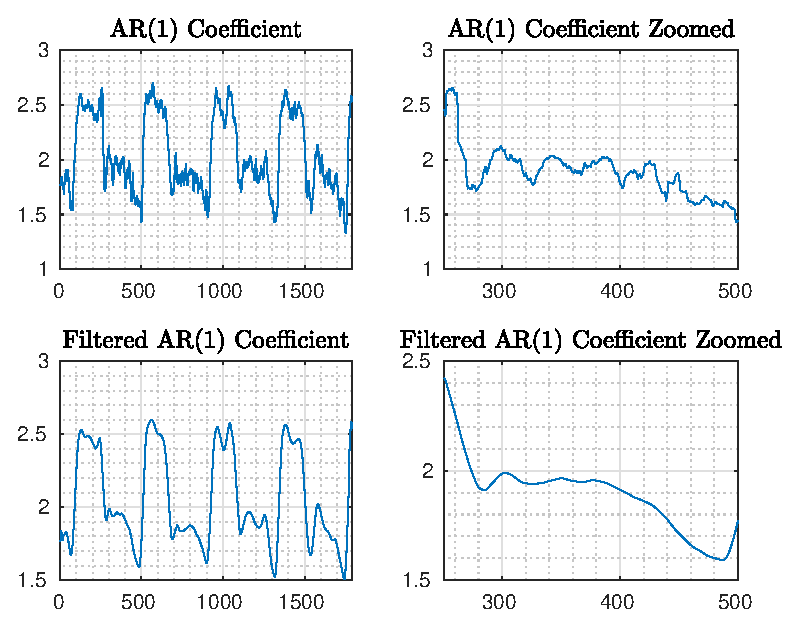
\includegraphics[width=\textwidth]{figures/prefiltering.eps}
		\caption{Filtering The Flow Estimate}
		\label{fig:prefiltering}
	\end{center}
\end{figure}
\subsection{Local Minima Extraction}
The number of local minima is decreased by filtering, however, it is still too much to process. So, we decided to add a heuristic algorithm to selection algorithm of local minima. We decided to use two types of local minimum, one type, let's call it $type$-1, is mostly seen in transition from expiration to inspiration and the other, $type$-2, is mostly seen in transition from inspiration to expiration. We don't expect any minima in the right neighborhood of $type$-1 minimum and in the left neighborhood of $type$-2 minimum for a certain amount of distance. 
The examples to $type$-1 and $type$-2 minima is shown in figure \ref{fig:minima}.
\begin{figure}
	\begin{center}
		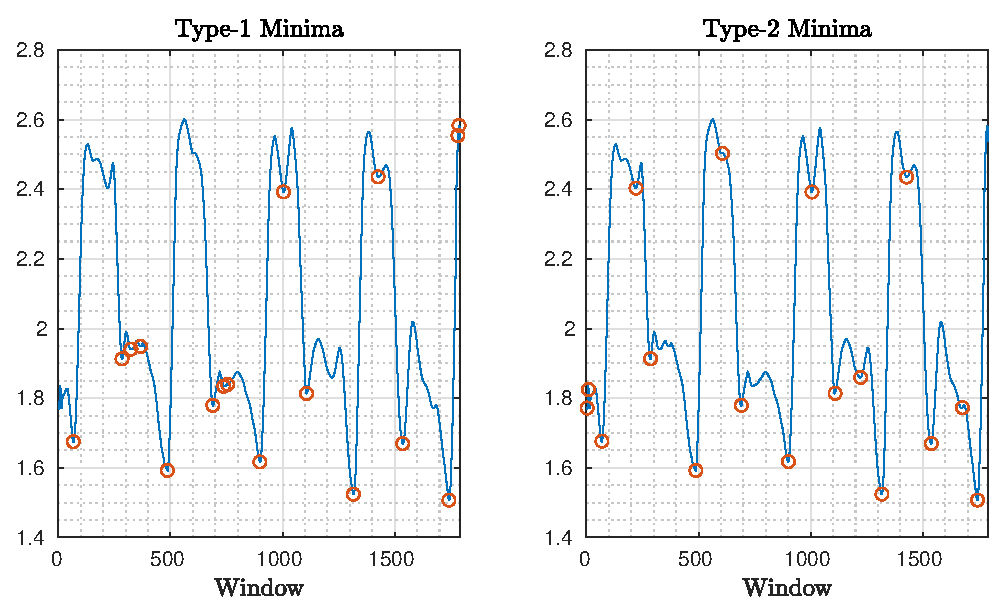
\includegraphics[width=\textwidth]{figures/minima.eps}
		\caption{Type-1 and Type-2 Minima}
		\label{fig:minima}
	\end{center}
\end{figure}
\subsection{Selection of Transition Points}
We use the period estimation and local minima together to decide on the location of transition points. While all the local minima are candidate transition points, we assume that the distribution of the distances between consecutive transitions from inspiration to expiration and expiration to inspiration have a distribution with a small variance and a mean which is equal to the period estimation. So, firstly, we decide on the number of transitions in each direction. Then we list all the subsets of local minima which has the number of transition elements. Finally we calculate the likelihoods of each subset according to \eqref{eq:likelihood} and select the one which has most. After selecting the first transition points set, in order to decide on the set belonging to the other transition type, we also look at the distance to the set of first transition type. In this method we don't assume any value for the duty cycle. An example of change point estimation is given in \ref{fig:transition}.
\begin{equation}
	L(\vec{d}) = \frac{\exp((\vec{d}-T')^T(\vec{d}-T')/\sigma^2)}{\sigma}
	\label{eq:likelihood} 
\end{equation}
\begin{figure}[h!]
	\begin{center}
		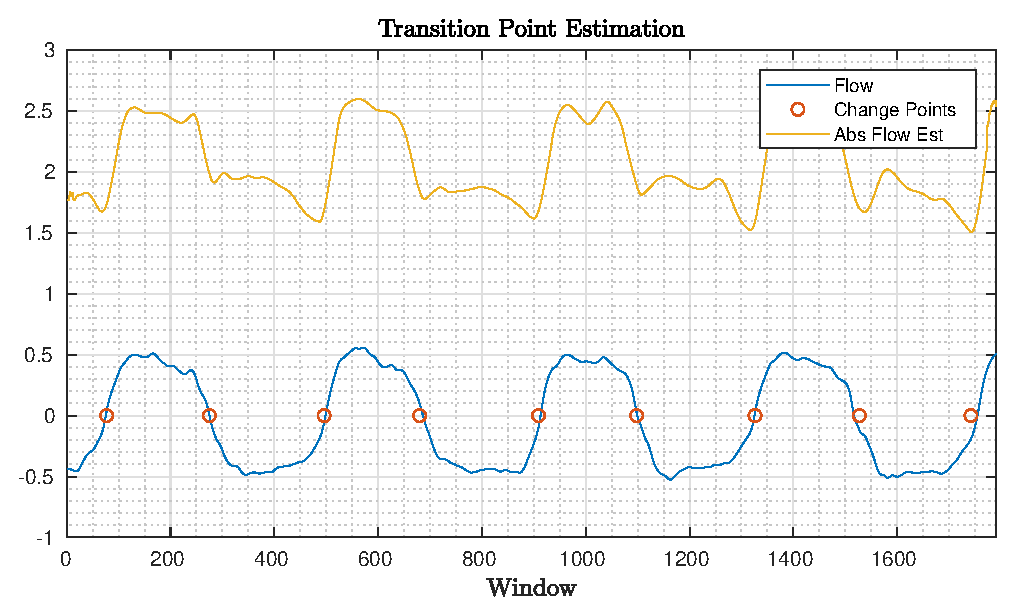
\includegraphics[width=\textwidth]{figures/transition.eps}
		\caption{Transition Point Estimation}
		\label{fig:transition}
	\end{center}
\end{figure}
\subsection{Estimating The Phases Given Transition Points}
We estimate the phases of segments after deciding on transition points by using the first AR coefficient of segments divided by the transitions points. We create two group and each group includes nonconsecutive segments. We then calculate the AR coefficients for each segment, and we label the group with a greater average AR coefficient as inspiration. This method works with a success rate of 96\%.